% Hand-polished LaTeX version following HW/00/docs/answer/latex/answer_indented.tex.
\documentclass[12pt,a4paper,fontset=none]{ctexart}

\usepackage[left=2.7cm,right=2.7cm,top=2.5cm,bottom=2.5cm]{geometry}
\usepackage{amsmath, amssymb}
\usepackage{booktabs}
\usepackage{longtable}
\usepackage{array}
\usepackage{calc}
\usepackage[font=small,labelfont=bf,labelsep=quad]{caption}
\usepackage{graphicx}
\usepackage{float}
\usepackage{hyperref}
\usepackage{xurl}
\usepackage{xcolor}
\usepackage{fancyvrb}
\usepackage{fvextra}
\usepackage{setspace}
\usepackage{enumitem}
\usepackage{etoolbox}

\let\OriginalIncludeGraphics\includegraphics
\renewcommand{\includegraphics}[2][]{%
  \OriginalIncludeGraphics[width=\linewidth,height=0.88\textheight,keepaspectratio,#1]{#2}%
}

\setmainfont{TeX Gyre Pagella}
\setCJKmainfont{Noto Serif CJK SC}
\setmonofont{DejaVu Sans Mono}
\setCJKmonofont{Noto Sans CJK SC}
\graphicspath{{../}{../assets/}{../../../result/}{../../../results/}{../../../outputs/}}
\setstretch{1.36}
\AtBeginDocument{\zihao{-4}\selectfont}
\setlength{\parindent}{2em}
\setlength{\parskip}{0pt}
\setlength{\abovedisplayskip}{0.65\baselineskip}
\setlength{\belowdisplayskip}{0.65\baselineskip}
\captionsetup{skip=0.35\baselineskip}
\sloppy
\clubpenalty=10000
\widowpenalty=10000

\hypersetup{
  hidelinks
}

\setcounter{secnumdepth}{3}
\setcounter{tocdepth}{2}
\renewcommand{\thesubsection}{\arabic{subsection}}
\renewcommand{\thesubsubsection}{\thesubsection.\arabic{subsubsection}}
\ctexset{
  subsection = {
    format = {\zihao{-3}\bfseries},
    aftername = {\quad},
    beforeskip = {1.0\baselineskip},
    afterskip = {0.45\baselineskip}
  },
  subsubsection = {
    format = {\zihao{4}\bfseries},
    aftername = {\quad},
    beforeskip = {0.75\baselineskip},
    afterskip = {0.25\baselineskip}
  }
}

\newcommand{\reportgroup}[1]{%
  \phantomsection\addcontentsline{toc}{section}{#1}%
  \begin{center}
    {\zihao{4}\bfseries #1\par}%
  \end{center}
  \vspace{0.65\baselineskip}%
}
\newcommand{\problem}[1]{\subsection{#1}}
\newcommand{\blocktitle}[1]{\subsubsection{#1}}
% 内联排版规则：
% 1. 正文内的英文、数字、短命令和路径应尽量保持同一正文字体，避免一段内混用多套字形。
% 2. \codeinline 只提供内联技术词标记，不切换到等宽字体；真正的命令片段放入 CodeBlock。
% 3. 普通数值和单位不要用 \texttt；直接使用正文，例如 0.0009765625 或 2 bytes。
% 4. 文件路径使用 \fileinline；它保持正文字体，并使用 URL 断行规则，避免长路径拉坏行距。
% 5. 正文公式、变量、等式和指数必须使用数学模式，例如 \(2^{-10}\)、\(1+t\)、\((1+t)^2-1\)、\(b=100\)；
%    不要写成 \texttt{2\^{}(-10)}、\texttt{1+t} 或 \texttt{(1+t)\^{}2-1}，否则只会按代码文本排版。
\newcommand{\codeinline}[1]{{\normalfont #1}}
\newcommand{\fileinline}[1]{{\urlstyle{same}\nolinkurl{#1}}}
\newcommand{\scriptpath}[1]{\fileinline{#1}}
\newcommand{\githubscriptsbase}{https://github.com/Void0312Aurora/computational-physics-homework-2026/blob/main/03/scripts}
\newcommand{\scriptlink}[1]{\noindent\textbf{相关脚本：}\href{../../../scripts/#1}{本地 \scriptpath{scripts/#1}} / \href{\githubscriptsbase/#1}{GitHub \scriptpath{scripts/#1}}\par\medskip}
\DefineVerbatimEnvironment{CodeBlock}{Verbatim}{
  fontsize=\footnotesize,
  frame=single,
  framesep=0.5em,
  xleftmargin=1.2em,
  xrightmargin=1.2em
}
\providecommand{\tightlist}{\setlength{\itemsep}{0pt}\setlength{\parskip}{0pt}}
\providecommand{\pandocbounded}[1]{#1}
\newcounter{none}
\newcommand{\passthrough}[1]{#1}
\setlist{nosep,leftmargin=2em}
\setlength{\LTpre}{0.35\baselineskip}
\setlength{\LTpost}{0.35\baselineskip}
\newif\ifwidetable
\newif\iftighttable
\setlength{\tabcolsep}{4pt}
\AtBeginEnvironment{longtable}{%
  \iftighttable
    \fontsize{6.7pt}{8.1pt}\selectfont\setlength{\tabcolsep}{0pt}%
  \else\ifwidetable
    \footnotesize\setlength{\tabcolsep}{2pt}%
  \else
    \normalsize\setlength{\tabcolsep}{4pt}%
  \fi\fi
  \renewcommand{\arraystretch}{1.16}%
  \renewcommand{\texttt}[1]{{\ttfamily #1}}%
}
\emergencystretch=3em

\title{\vspace{-1.0em}{\bfseries\zihao{3} Homework 4}\\[0.35em]{\zihao{-4} 数值稳定性分析报告}}
\author{\zihao{-4} 姜玥晟}
\date{\zihao{-4} 2026-04-21}

\begin{document}
\pagestyle{plain}
\maketitle

\begin{figure}[H]
  \centering
  
\includegraphics[width=0.18\linewidth]{profile.jpg}
\end{figure}

\begin{table}[H]
  \centering
  \begin{tabular}{>{\raggedright\arraybackslash}p{0.20\linewidth}>{\raggedright\arraybackslash}p{0.64\linewidth}}
    \toprule
    项目 & 内容 \\
    \midrule
    源题编号 & \codeinline{HW04} \\
    学生姓名 & 姜玥晟 \\
    报告主题 & 二次方程求根稳定性、多项式求值稳定性与 half precision 舍入误差 \\
    实验环境 & \codeinline{C} 数值程序与 \codeinline{Python} 统计绘图程序 \\
    \bottomrule
  \end{tabular}
\end{table}

\newpage

\renewcommand{\contentsname}{目录}
\begingroup
\hypersetup{linkcolor=black}
\tableofcontents
\thispagestyle{plain}
\endgroup

\newpage

\reportgroup{I. 二次方程小根的相消误差分析}

考察二次方程

\[
x^2 - b x + 1 = 0,
\]

其两根可写为

\[
x_1 = \frac{b+r}{2}, \qquad
x_2 = \frac{b-r}{2}, \qquad
r = \sqrt{b^2 - 4}.
\]

当 \(b\) 足够大时，\(r\) 与 \(b\) 的数值非常接近，小根

\[
x_2 = \frac{b-r}{2}
\]

的计算将涉及两个接近量之间的相减。

\subsection{\texorpdfstring{Problem 1(1)：\(b=100\) 附近的误差考察}{Problem 1(1)：b=100 附近的误差考察}}\label{problem-11b100-ux9644ux8fd1ux7684ux8befux5deeux8003ux5bdf}

\scriptlink{problem1.c}

\blocktitle{待求问题}

首先考察该表达式在 \(b=100\) 附近的相对误差。

\blocktitle{解决方式}

为使实验步骤表达得更规范，本文以伪代码方式给出求解过程：

\begin{CodeBlock}
Input : precisions P, b = 100
Output: standard-form error at b = 100

for each p in P do
    r <- sqrt(b^2 - 4)
    x_std <- (b - r) / 2
    x_ref <- ref_root(b)
    err_std <- relerr(x_std, x_ref)
end for
\end{CodeBlock}

其中 \codeinline{ref\_root(b)} 表示高精度参考解，\codeinline{relerr} 表示相对误差计算函数。

\blocktitle{问题答案}

对于题目指定的 \(b=100\)，本机 IEEE \codeinline{float} 运算给出

\[
x_2^{\text{standard}} = 0.0100021362,
\]

高精度参考值约为 \(0.010001000200050014\)。标准公式相对误差为 1.1359E-4。

题图第二页另给出 \(b=97\) 的三位有效数字教学示例：

\[
x_2^{\text{exact}} = 0.01031, \qquad
x_2^{\text{standard}} = 0.01050,
\]

该示例的相对误差为 1.8429E-2，约为 \(1.84\%\)，用于说明低精度三位有效数字运算中的相消误差；它不是 \(b=100\) 的主计算结果。

\blocktitle{分析}

标准公式的不稳定性来源于相消误差。由近似关系

\[
\sqrt{b^2-4} = b\sqrt{1-4/b^2} \approx b - \frac{2}{b}
\]

可知，当 \(b\) 很大时，表达式

\[
b - \sqrt{b^2 - 4}
\]

仅保留数量级约为 \(2/b\) 的小量，高位有效数字会在减法阶段被提前消耗。因此，本问只能说明标准公式已经出现相消误差；如何通过代数改写避开该相减过程，留到 Problem 1(3) 再处理。

\subsection{Problem 1(2)：大参数区间的误差比较}\label{problem-12ux5927ux53c2ux6570ux533aux95f4ux7684ux8befux5deeux6bd4ux8f83}

\scriptlink{problem1.c}

\blocktitle{待求问题}

随后增大 \(b\) 取值并列表比较误差变化。

\blocktitle{解决方式}

为使实验步骤表达得更规范，本文以伪代码方式给出求解过程：

\begin{CodeBlock}
Input : precisions P, test values B
Output: standard-form error table

for each p in P do
    for each b in B do
        r <- sqrt(b^2 - 4)
        x_std <- (b - r) / 2
        x_ref <- ref_root(b)
        err_std <- relerr(x_std, x_ref)
    end for
end for
\end{CodeBlock}

其中 \codeinline{ref\_root(b)} 表示高精度参考解，\codeinline{relerr} 表示相对误差计算函数。

\blocktitle{问题答案}

继续增大 \(b\) 并仍然只使用标准公式 \(x_2=(b-r)/2\) 时，代表性相对误差如下。

{\def\LTcaptype{none} % do not increment counter
\begin{longtable}[]{@{}lrr@{}}
\toprule\noalign{}
精度 & b & 标准公式相对误差 \\
\midrule\noalign{}
\endhead
\bottomrule\noalign{}
\endlastfoot
float & 100 & 1.1359E-4 \\
float & 1000 & 7.0791E-3 \\
float & 10000 & 1.0000E+0 \\
double & 100000 & 3.3844E-7 \\
double & 10000000000 & 1.0000E+0 \\
quad & 10000000000 & 6.8266E-16 \\
\end{longtable}
}

对于 \codeinline{float}，当 \(b=10000\) 时，标准公式的相对误差已达到 1.0000E+0，说明小根信息几乎完全丢失。对于 \codeinline{double}，在 \(b=10^{10}\) 时也出现同类退化，而 \codeinline{\_\_float128} 在同一测试点仍维持 6.8266E-16 的误差量级。

\blocktitle{分析}

标准公式的不稳定性来源于相消误差。由近似关系

\[
\sqrt{b^2-4} = b\sqrt{1-4/b^2} \approx b - \frac{2}{b}
\]

可知，当 \(b\) 很大时，表达式

\[
b - \sqrt{b^2 - 4}
\]

仅保留数量级约为 \(2/b\) 的小量，高位有效数字会在减法阶段被提前消耗。表中的退化正是这一相消过程随 \(b\) 增大而加剧的结果。下一问再对这个表达式进行代数改写，并用同一组 \(b\) 值复现实验。

\subsection{Problem 1(3)：有理化改写与再实验}\label{problem-13ux6709ux7406ux5316ux6539ux5199ux4e0eux518dux5b9eux9a8c}

\scriptlink{problem1.c}

\blocktitle{待求问题}

最后将小根公式改写为

\[
x_2 = \frac{(b-r)(b+r)}{2(b+r)} = \frac{2}{b+r},
\]

并重新进行同样的实验，以比较两种实现的稳定性差异。

\blocktitle{解决方式}

为使实验步骤表达得更规范，本文以伪代码方式给出求解过程：

\begin{CodeBlock}
Input : precisions P, test values B
Output: error table and error curve

for each p in P do
    for each b in B do
        r <- sqrt(b^2 - 4)
        x_std <- (b - r) / 2
        x_rat <- 2 / (b + r)
        x_ref <- ref_root(b)
        err_std <- relerr(x_std, x_ref)
        err_rat <- relerr(x_rat, x_ref)
    end for
end for
\end{CodeBlock}

其中 \codeinline{ref\_root(b)} 表示高精度参考解，\codeinline{relerr} 表示相对误差计算函数。

\blocktitle{问题答案}

对同一组 \(b\) 值重新实验后，代表性结果如下。

\begin{figure}[H]
\centering
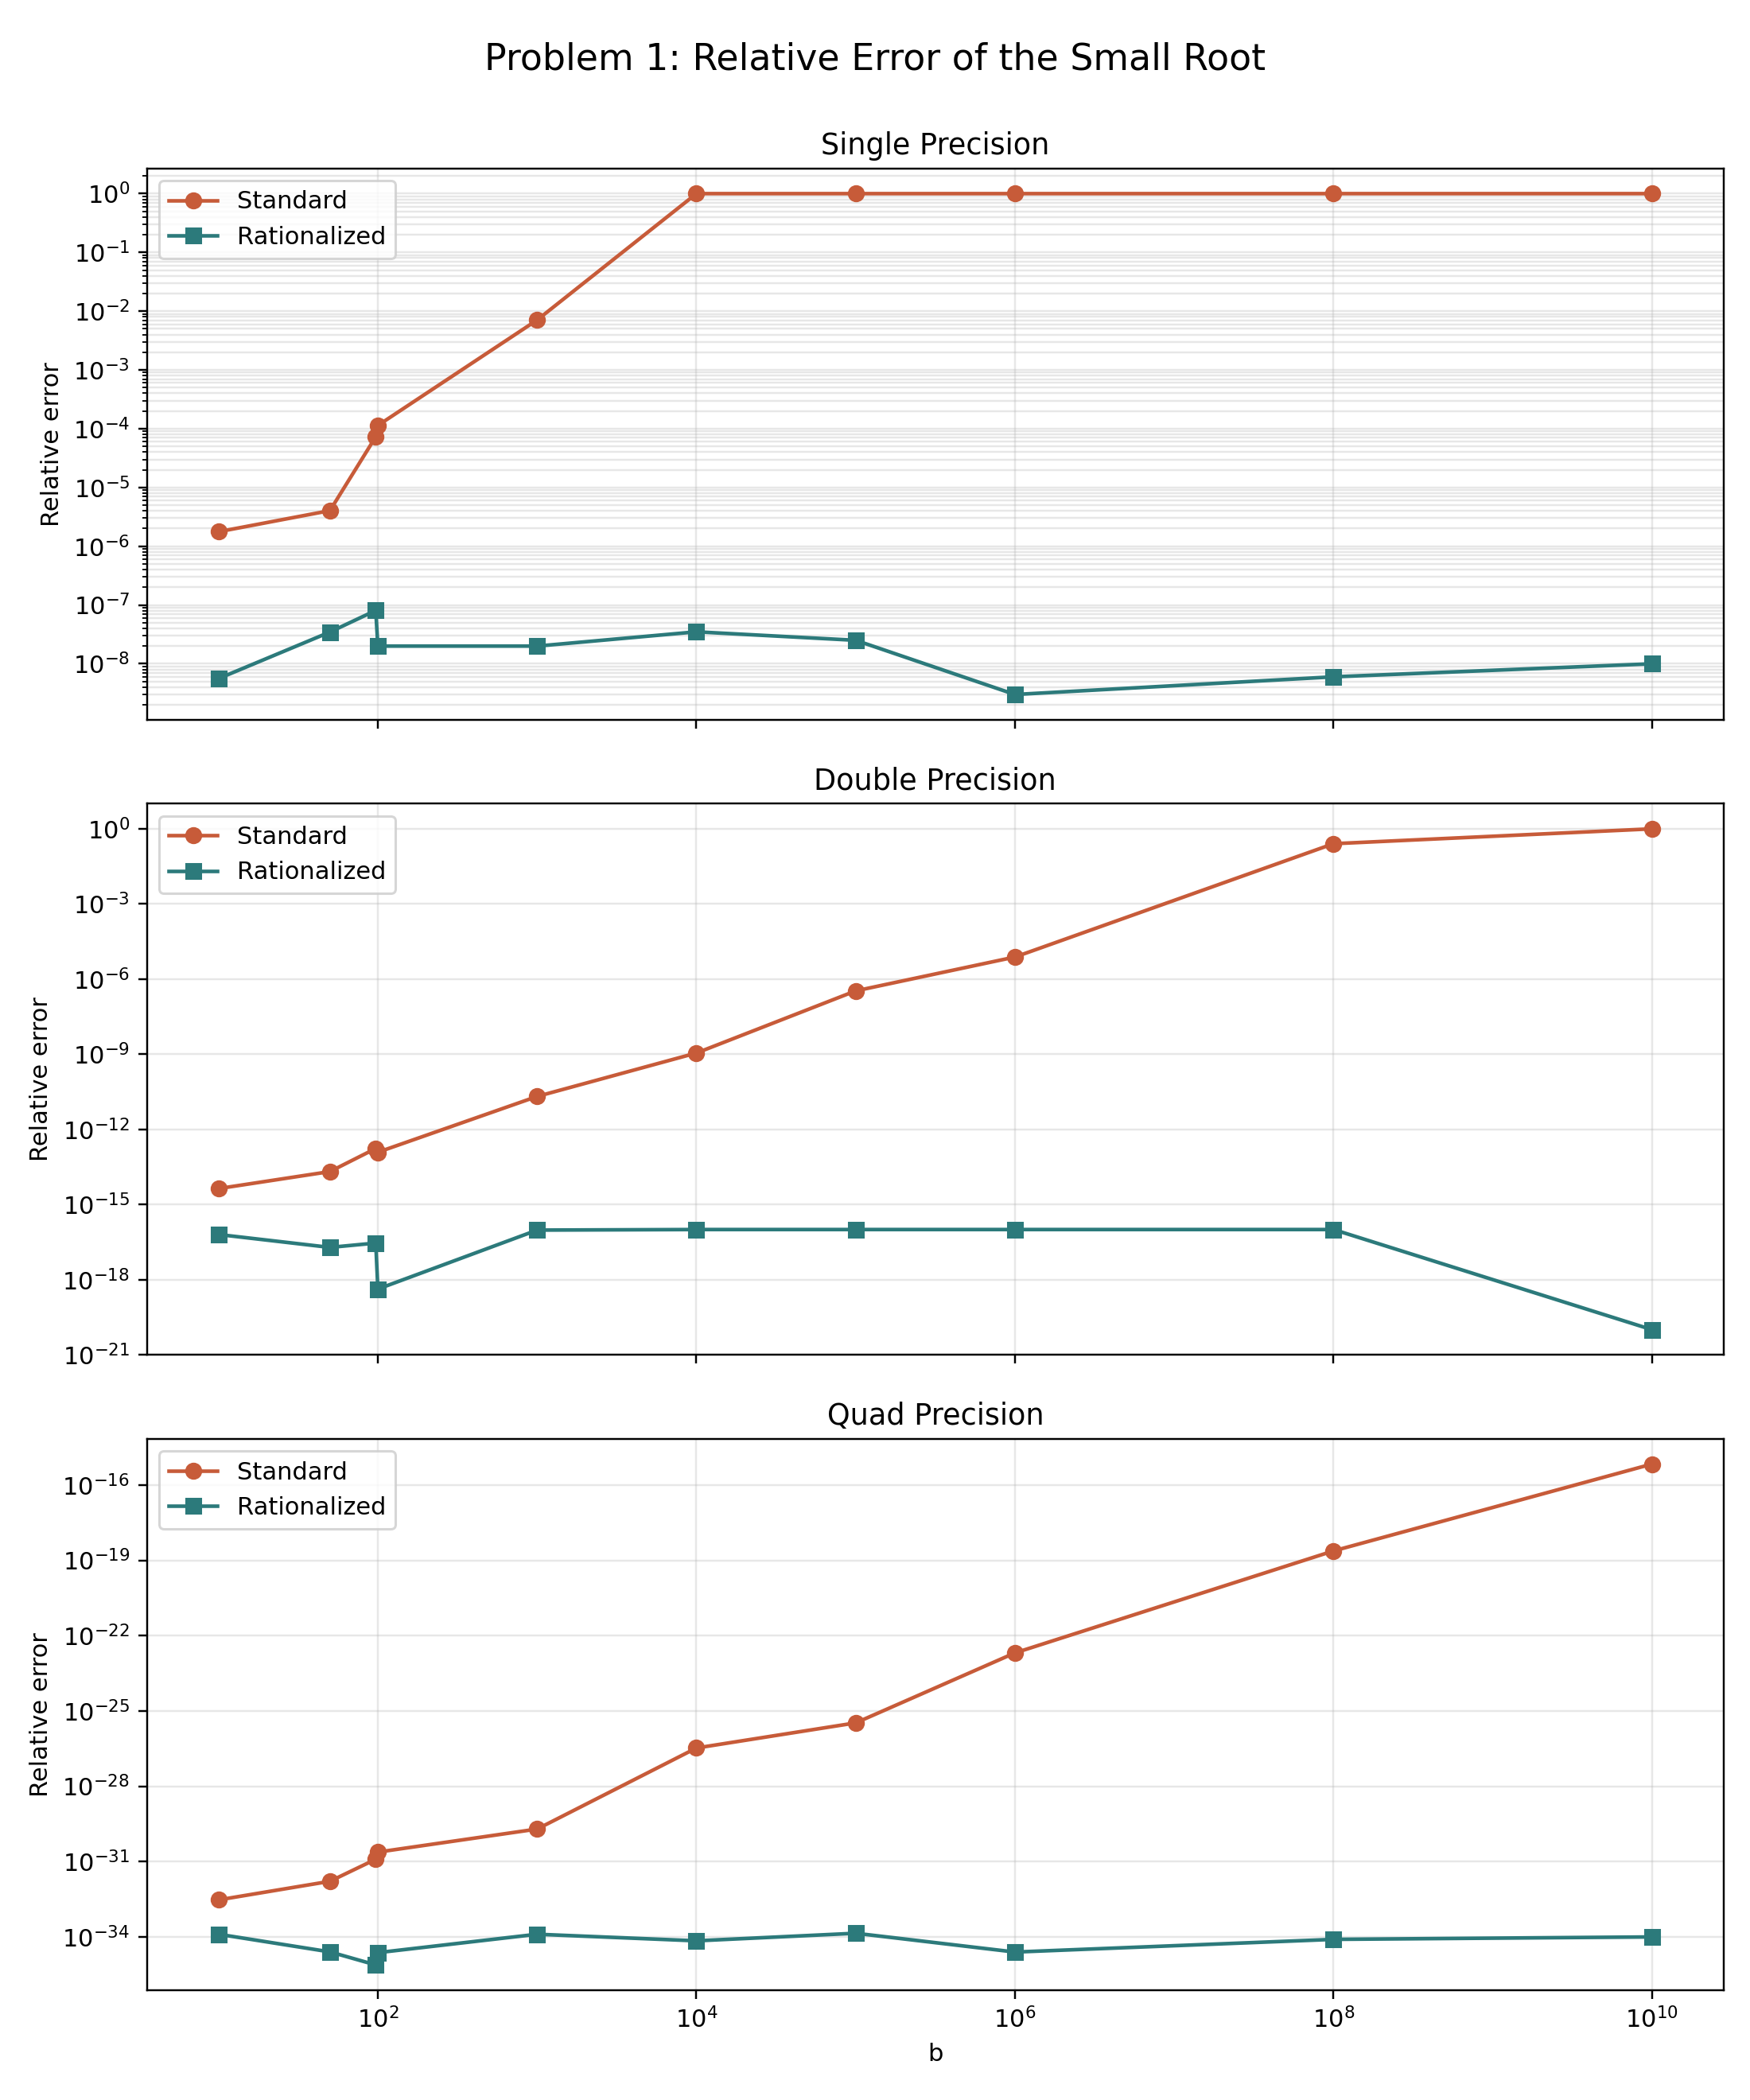
\includegraphics[width=0.88\linewidth,height=0.78\textheight,keepaspectratio,alt={Problem 1 relative-error comparison after rationalization}]{../../../result/problem1_relative_error.png}
\caption{Problem 1 relative-error comparison after rationalization}
\end{figure}

{\def\LTcaptype{none} % do not increment counter
\begin{longtable}[]{@{}lrrrr@{}}
\toprule\noalign{}
精度 & b & 标准公式相对误差 & 有理化公式相对误差 & 改进倍数 \\
\midrule\noalign{}
\endhead
\bottomrule\noalign{}
\endlastfoot
float & 100 & 1.1359E-4 & 2.0003E-8 & 5.6786E+3 \\
float & 1000 & 7.0791E-3 & 2.0002E-8 & 3.5392E+5 \\
float & 10000 & 1.0000E+0 & 3.5000E-8 & 2.8571E+7 \\
double & 100000 & 3.3844E-7 & 9.9980E-17 & 3.3850E+9 \\
double & 10000000000 & 1.0000E+0 & 1.0000E-20 & 1.0000E+20 \\
quad & 10000000000 & 6.8266E-16 & 1.0000E-34 & 6.8266E+18 \\
\end{longtable}
}

这些数据说明，有理化后未再出现与标准公式同量级的误差爆炸。实验范围内，有理化公式始终显著优于标准公式；例如在 \codeinline{double} 且 \(b=10^{10}\) 条件下，标准公式误差为 1.0000E+0，而有理化公式误差为 1.0000E-20。

\blocktitle{分析}

标准公式的不稳定性来源于相消误差。由近似关系

\[
\sqrt{b^2-4} = b\sqrt{1-4/b^2} \approx b - \frac{2}{b}
\]

可知，当 \(b\) 很大时，表达式

\[
b - \sqrt{b^2 - 4}
\]

仅保留数量级约为 \(2/b\) 的小量，高位有效数字会在减法阶段被提前消耗。有理化公式

\[
x_2 = \frac{2}{b + \sqrt{b^2 - 4}}
\]

将这一相减过程替换为除法运算，因此显著抑制了误差放大。进一步地，由根的乘积关系 \(x_1 x_2 = 1\) 还可得到另一种稳定实现，即先稳定计算较大的根 \(x_1\)，再由 \(x_2 = 1/x_1\) 得到小根。

\reportgroup{II. 多项式写法对数值稳定性的影响}

作业要求在 \codeinline{single}、\codeinline{double} 与 \codeinline{quad} 三种精度下计算

\[
(x-1)^{10}
\]

及其多项式展开式，并在区间 \(x\in[0.7, 1.3]\) 上观察数值结果。

\subsection{Problem 2(1)：局部放大观察}\label{problem-21ux5c40ux90e8ux653eux5927ux89c2ux5bdf}

\scriptlink{problem2.c}

\blocktitle{待求问题}

比较直接形式与展开形式在局部区间上的数值表现。

\blocktitle{解决方式}

本题的实验组织可形式化表示为：

\begin{CodeBlock}
Input : grid X, methods M, precisions P
Output: zoomed plots and error statistics

for each p in P do
    for each x in X do
        y_ref <- high_precision((x - 1)^10)
        for each m in M do
            y <- eval(m, x, p)
            if y_ref != 0 then
                err[m, x, p] <- relerr(y, y_ref)
            end if
        end for
    end for
end for
\end{CodeBlock}

其中 \(M=\{\mathrm{direct},\mathrm{expanded},\mathrm{horner}\}\)，并基于 \codeinline{err} 进一步统计最大误差、峰值位置与中位误差。

\blocktitle{问题答案}

局部放大结果表明，直接形式在三个精度下均最接近参考曲线，而展开形式与 Horner 形式在 \(x=1\) 附近出现明显偏离。

\begin{figure}[H]
\centering
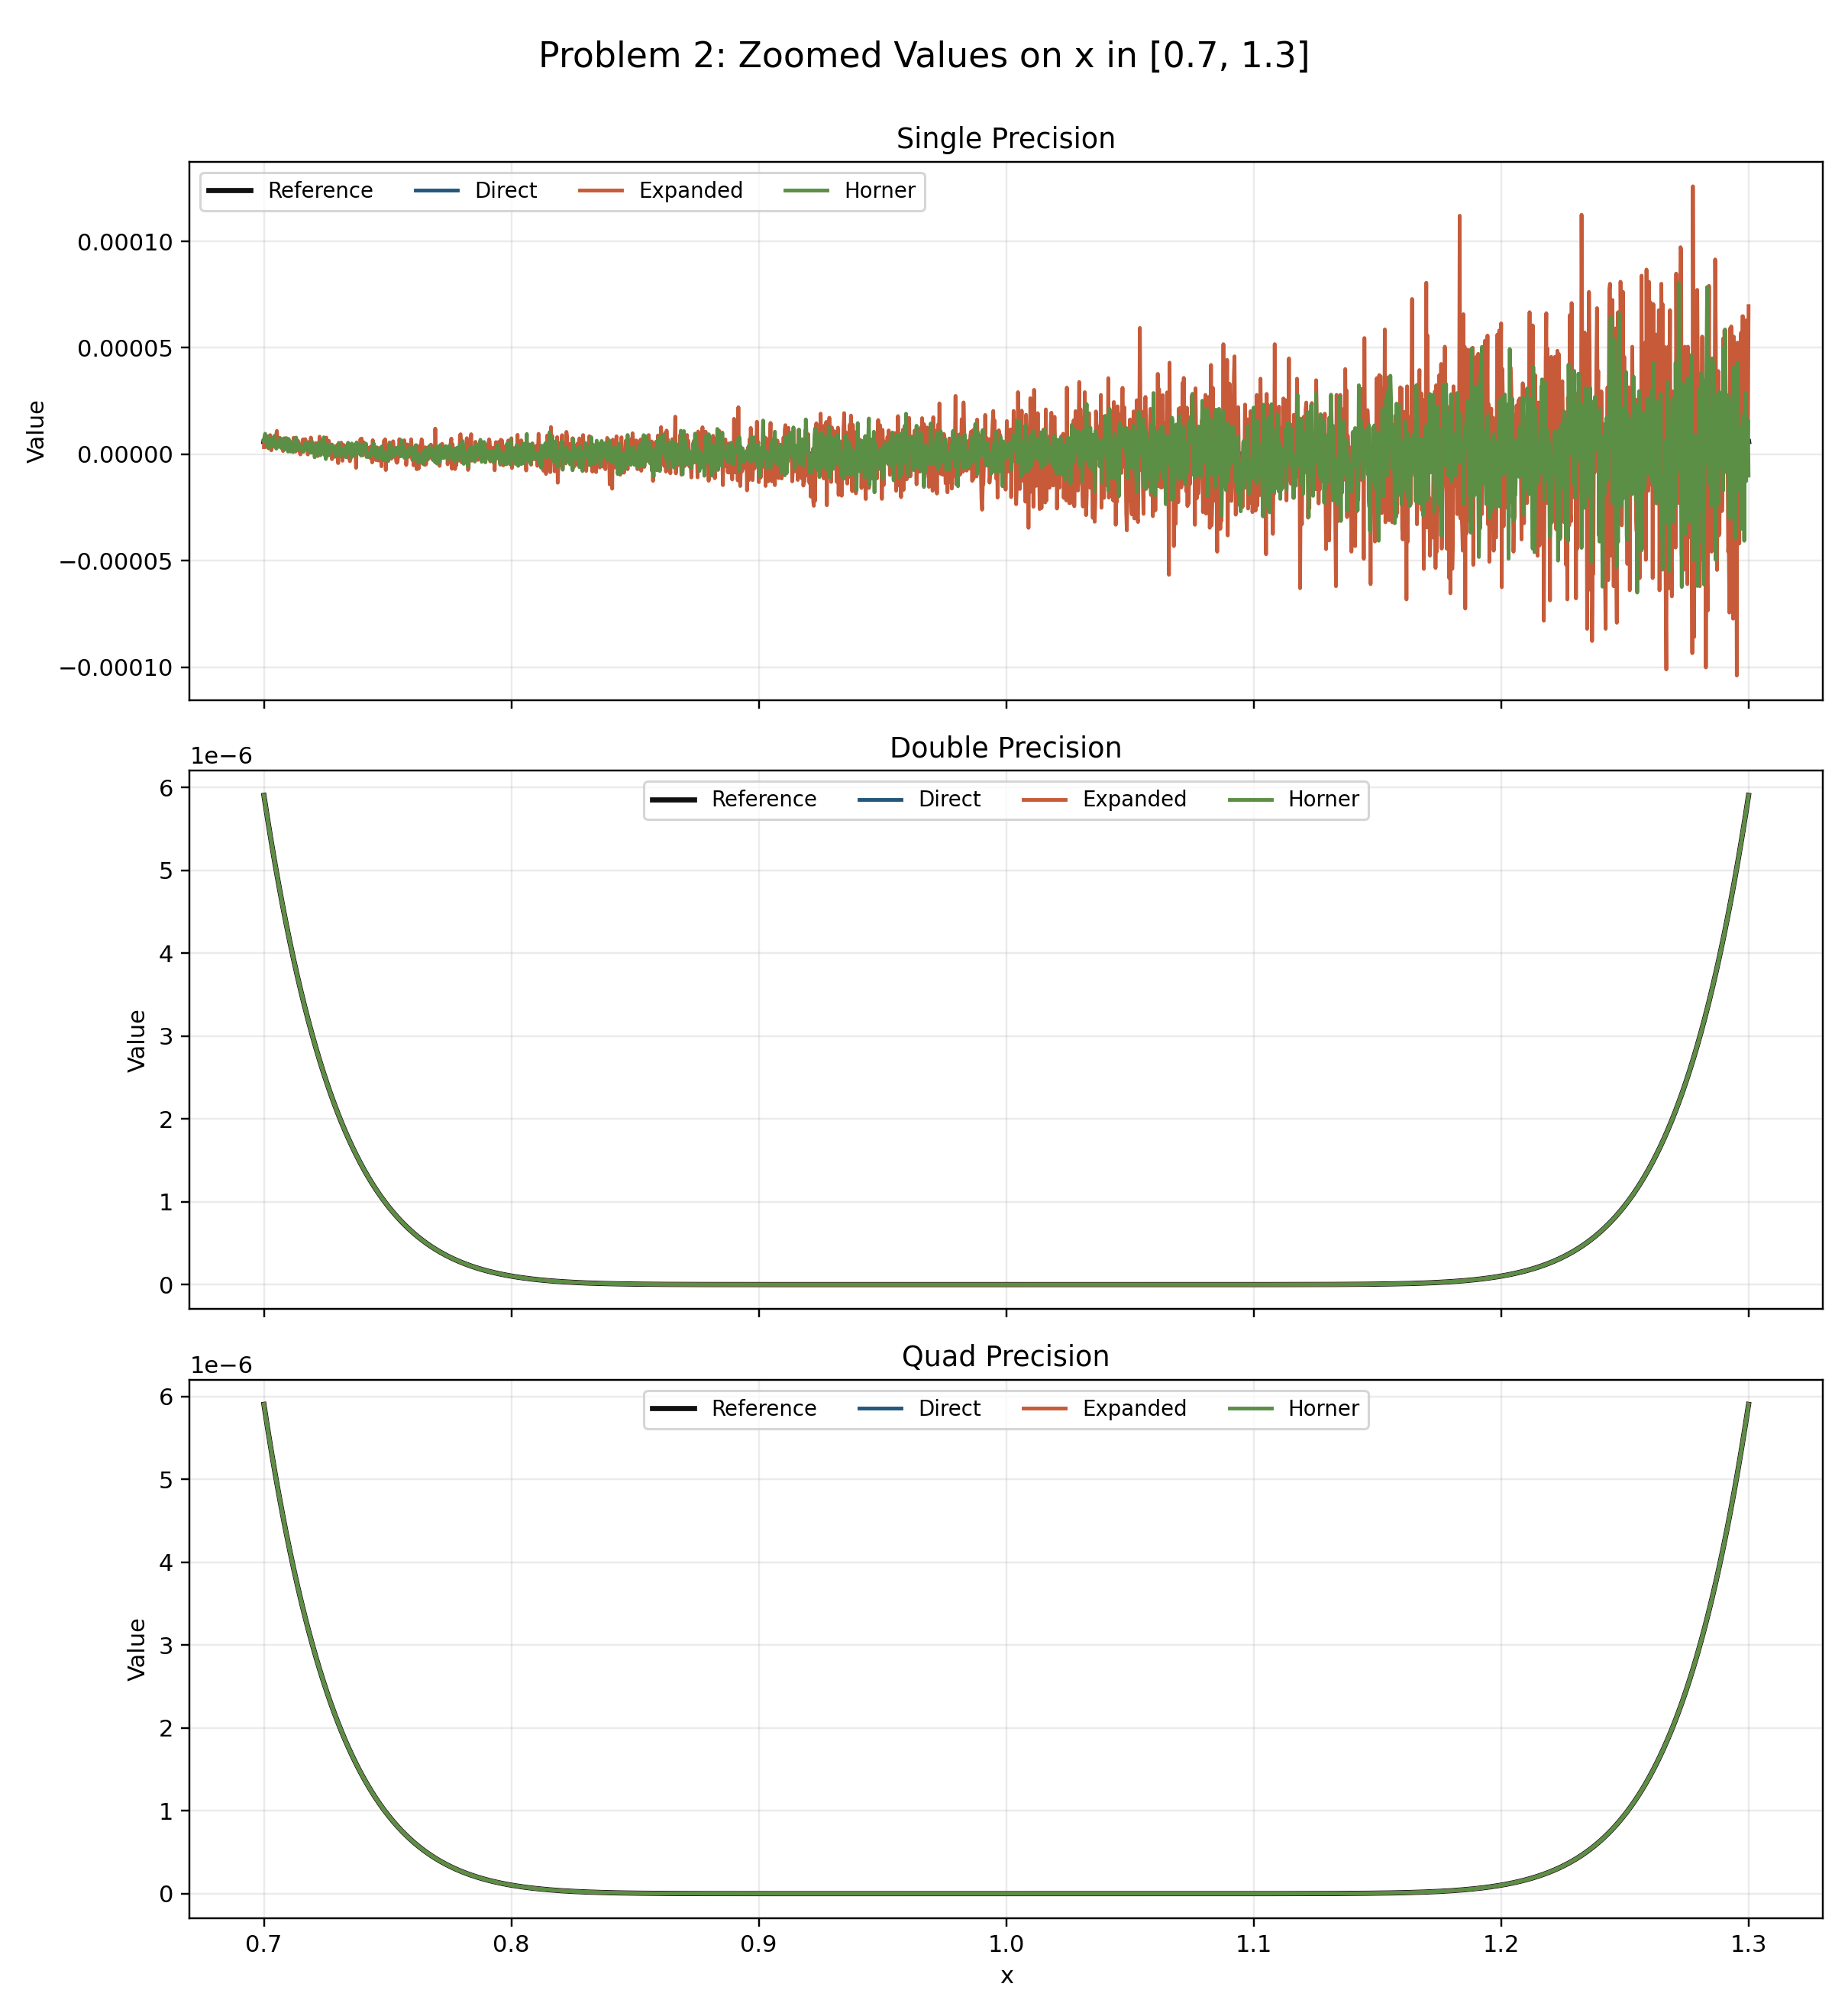
\includegraphics[width=0.88\linewidth,height=0.78\textheight,keepaspectratio,alt={Problem 2 zoomed-value comparison}]{../../../result/problem2_zoom.png}
\caption{Problem 2 zoomed-value comparison}
\end{figure}

造成该现象的直接原因在于：当 \(x\) 接近 \(1\) 时，真值 \((x-1)^{10}\) 极小；若先将多项式展开为多个数量级接近的项再相加减，就会显著放大舍入误差。

\blocktitle{分析}

本小问关注的是局部曲线形状。直接形式先计算 \(u=x-1\)，再计算 \(u^{10}\)，整个过程中被反复相乘的是接近零的小量；因此它能保留函数在 \(x=1\) 附近的平滑谷底。展开式则把同一个函数写成

\[
x^{10}-10x^9+45x^8-\cdots-10x+1,
\]

在 \(x\approx 1\) 时，上式各项本身仍是 \(O(1)\) 量级，最后却要抵消成 \(O(\lvert x-1\rvert^{10})\) 的极小结果。局部放大图中展开式曲线偏离参考曲线，说明问题不在函数本身，而在表达式写法引入了大数相减。

\subsection{Problem 2(2)：相对误差分布}\label{problem-22ux76f8ux5bf9ux8befux5deeux5206ux5e03}

\scriptlink{problem2.c}

\blocktitle{待求问题}

绘制并比较误差分布。

\blocktitle{解决方式}

本题的实验组织可形式化表示为：

\begin{CodeBlock}
Input : grid X, methods M, precisions P
Output: zoomed plots and error statistics

for each p in P do
    for each x in X do
        y_ref <- high_precision((x - 1)^10)
        for each m in M do
            y <- eval(m, x, p)
            if y_ref != 0 then
                err[m, x, p] <- relerr(y, y_ref)
            end if
        end for
    end for
end for
\end{CodeBlock}

其中 \(M=\{\mathrm{direct},\mathrm{expanded},\mathrm{horner}\}\)，并基于 \codeinline{err} 进一步统计最大误差、峰值位置与中位误差。

\blocktitle{问题答案}

相对误差统计结果如下。图中使用离散采样点而非折线连接；靠近 \(x=1\) 的针状峰来自相对误差分母 \(\lvert(x-1)^{10}\rvert\) 极小，少量绝对舍入误差被放大。相邻采样点误差可差多个数量级，若用折线连接会产生视觉上的竖直突变线，因此这里展示采样分布而不把它解释成连续曲线突变。

\begin{figure}[H]
\centering
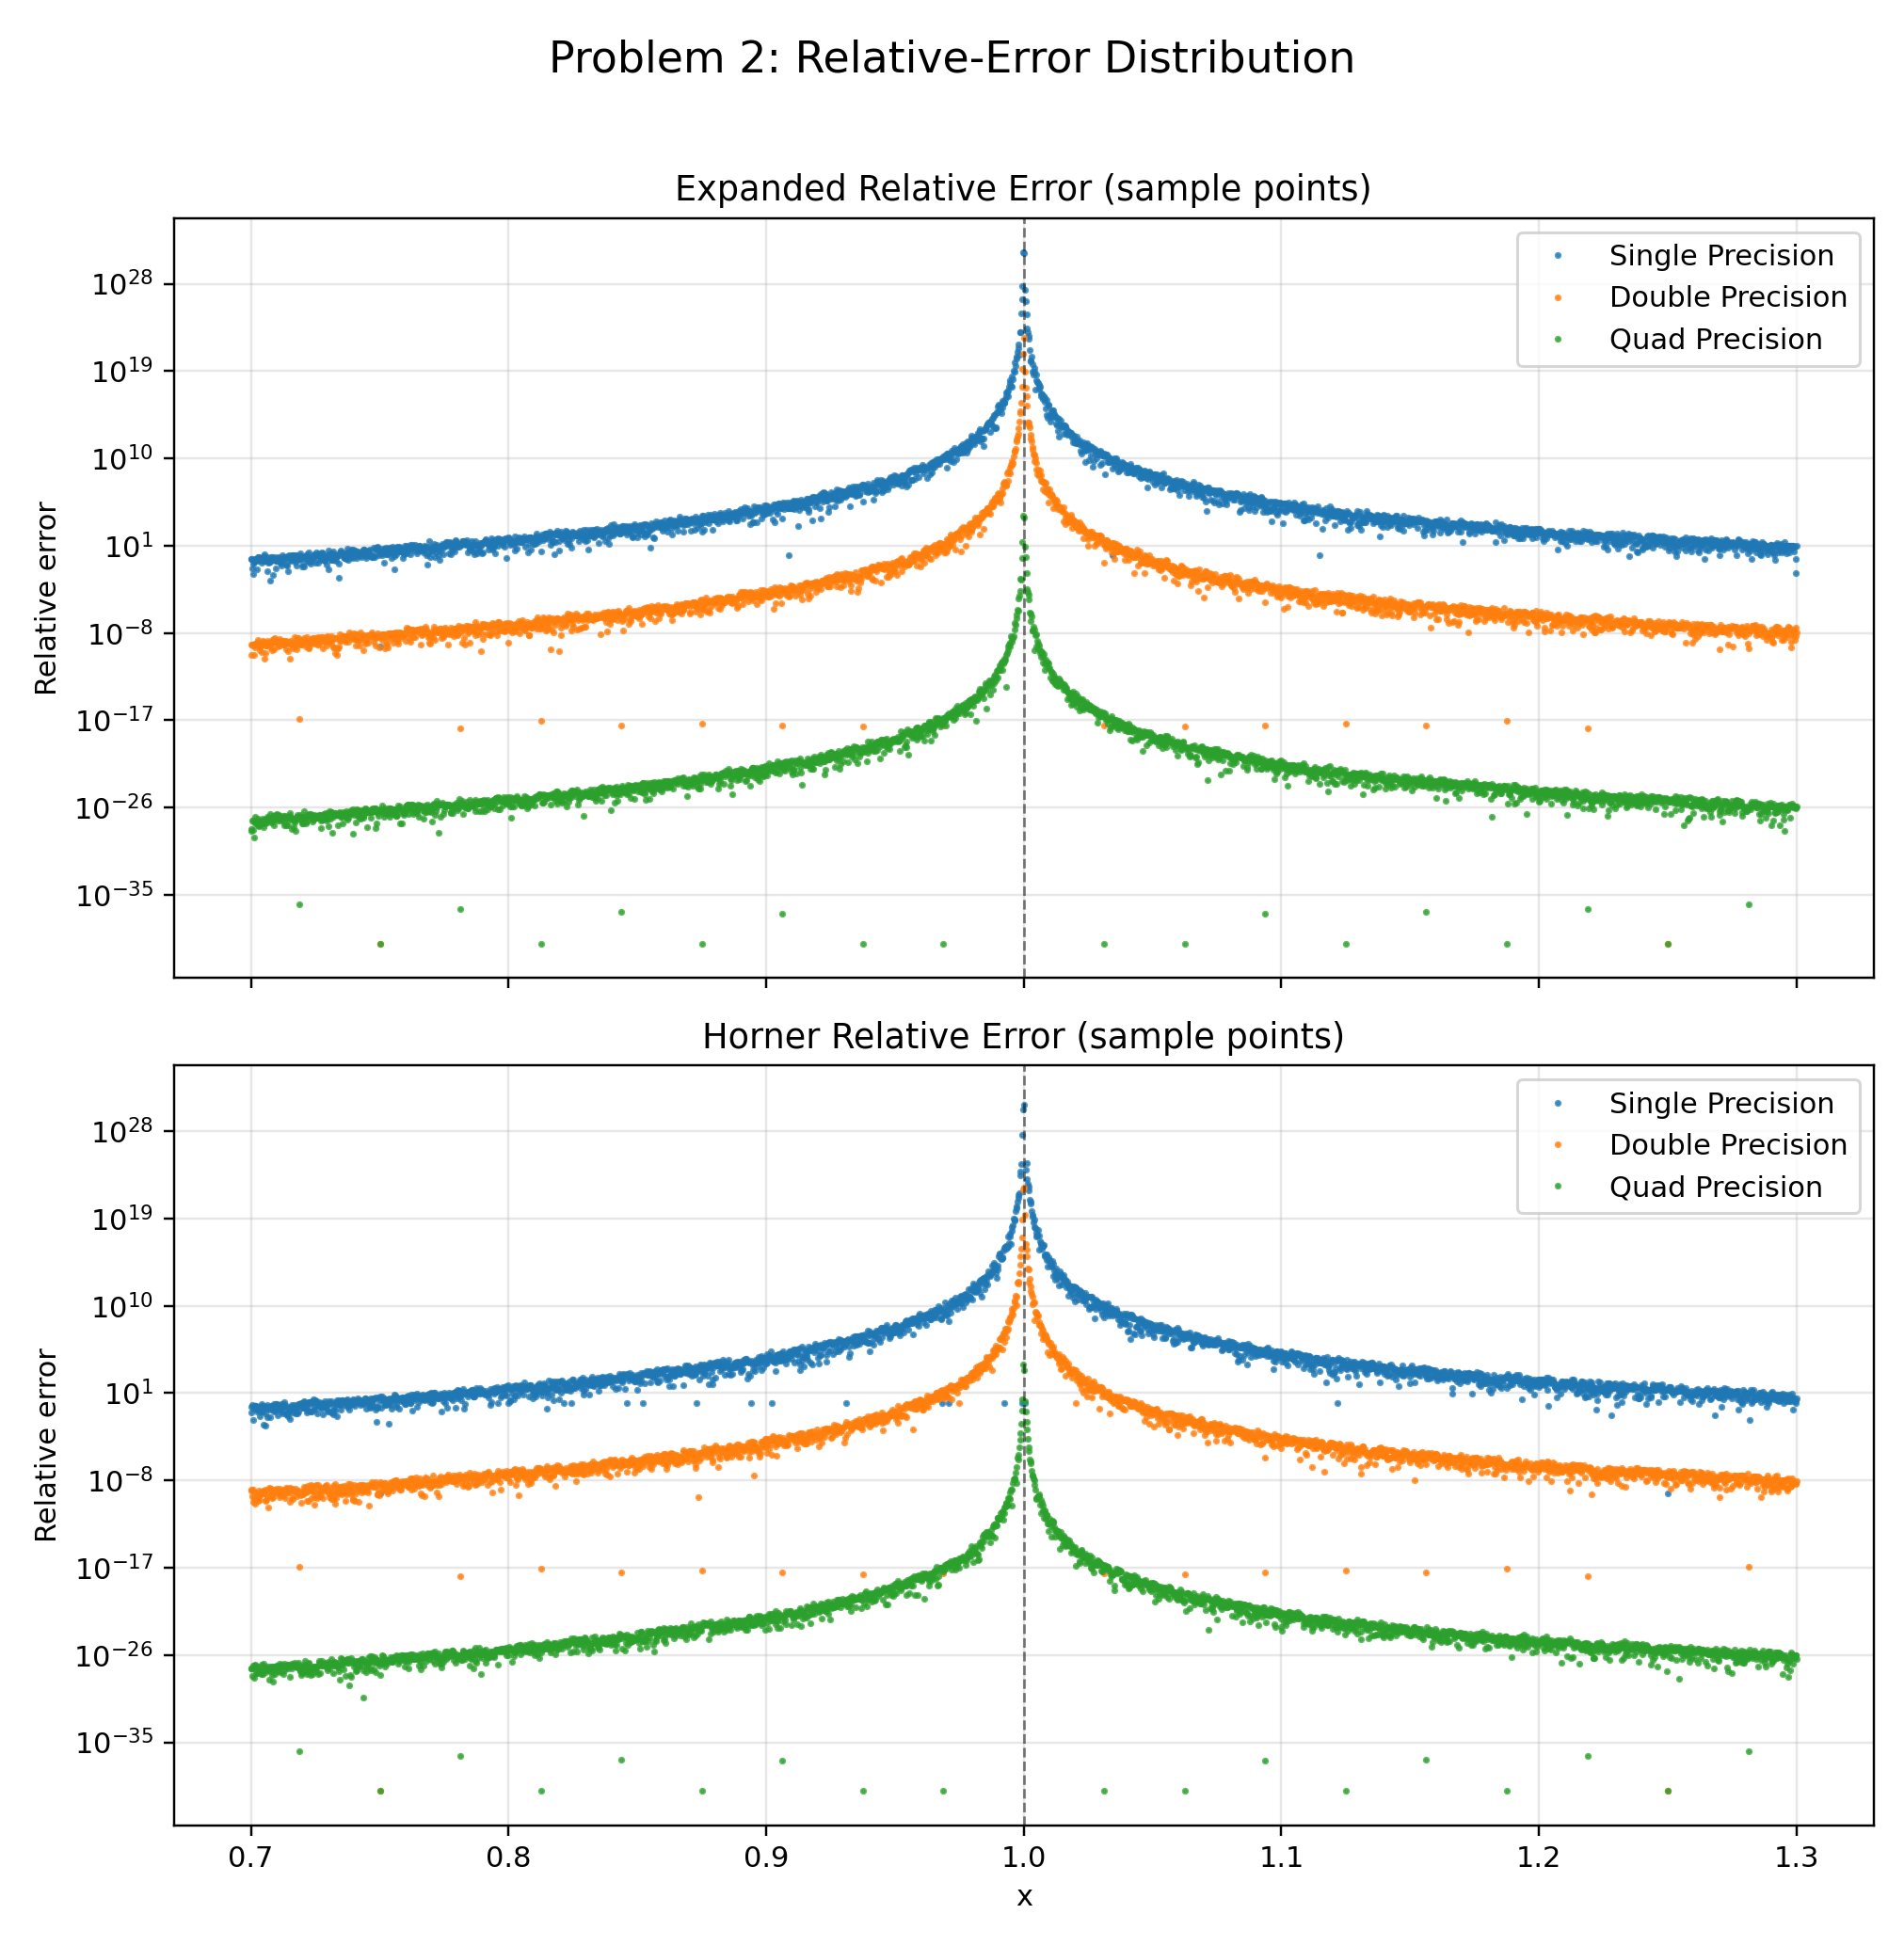
\includegraphics[width=0.96\linewidth,height=0.84\textheight,keepaspectratio,alt={Problem 2 relative-error distribution}]{../../../result/problem2_relative_error.png}
\caption{Problem 2 relative-error distribution}
\end{figure}

{\def\LTcaptype{none} % do not increment counter
\begin{longtable}[]{@{}llrrr@{}}
\toprule\noalign{}
精度 & 形式 & 最大相对误差 & 峰值位置 x & 中位相对误差 \\
\midrule\noalign{}
\endhead
\bottomrule\noalign{}
\endlastfoot
float & direct & 7.5107E-5 & 1.0005 & 9.5128E-8 \\
float & expanded & 1.7450E+31 & 0.99975002 & 1.3713E+3 \\
float & horner & 4.9415E+30 & 1.00025 & 7.3785E+2 \\
double & direct & 8.9867E-13 & 1.0005 & 5.2885E-16 \\
double & expanded & 2.6543E+22 & 1.00025 & 2.4256E-6 \\
double & horner & 1.4552E+22 & 1.00025 & 1.4286E-6 \\
quad & direct & 1.8490E-31 & 1.00025 & 1.2808E-34 \\
quad & expanded & 1.2522E+4 & 0.99975 & 2.3220E-24 \\
quad & horner & 9.3896E+3 & 0.99975 & 1.3699E-24 \\
\end{longtable}
}

其中最显著的退化出现在 \codeinline{float} 精度的 \codeinline{expanded} 形式，其最大相对误差达到 1.7450E+31，峰值出现在 \(x=0.99975002\) 附近。相比之下，\codeinline{float} 精度的直接形式最大相对误差仅为 7.5107E-5。即使在 \codeinline{quad} 精度下，展开形式的最大相对误差仍达到 1.2522E+4，说明表达式结构对稳定性的影响并不会因精度提升而完全消失。

\blocktitle{分析}

本小问关注的是相对误差的分布，而不是函数值本身。相对误差按

\[
\mathrm{relerr}(x)=\frac{\lvert y(x)-y_{\mathrm{ref}}(x)\rvert}{\lvert y_{\mathrm{ref}}(x)\rvert}
\]

计算；当 \(x\) 靠近 \(1\) 时，参考值 \(y_{\mathrm{ref}}=(x-1)^{10}\) 极小，所以即使绝对误差只有 \(10^{-14}\) 或 \(10^{-6}\)，也会被分母放大到很高的相对误差。统计表中的峰值位置均集中在 \(x=1\) 附近，例如 \codeinline{float + expanded} 的峰值在 \(x=0.99975002\)，最大相对误差达到 1.7450E+31。图中的针状峰因此是相对误差定义和采样点共同造成的结果，不应理解为原函数出现了真实间断。

\subsection{Problem 2(3)：Horner 方法比较}\label{problem-23horner-ux65b9ux6cd5ux6bd4ux8f83}

\scriptlink{problem2.c}

\blocktitle{待求问题}

再使用 Horner 方法重新组织多项式计算，比较三种实现的误差分布，并解释在 \(x=1\) 邻域出现差异的原因。

\blocktitle{解决方式}

本题的实验组织可形式化表示为：

\begin{CodeBlock}
Input : grid X, methods M, precisions P
Output: zoomed plots and error statistics

for each p in P do
    for each x in X do
        y_ref <- high_precision((x - 1)^10)
        for each m in M do
            y <- eval(m, x, p)
            if y_ref != 0 then
                err[m, x, p] <- relerr(y, y_ref)
            end if
        end for
    end for
end for
\end{CodeBlock}

其中 \(M=\{\mathrm{direct},\mathrm{expanded},\mathrm{horner}\}\)，并基于 \codeinline{err} 进一步统计最大误差、峰值位置与中位误差。

\blocktitle{问题答案}

Horner 方法的独立对比结果如下。表中``最大误差改善倍数''和``中位误差改善倍数''均定义为 \codeinline{expanded} 误差除以 \codeinline{horner} 误差；数值大于 \(1\) 表示 Horner 优于朴素展开。

{\def\LTcaptype{none} % do not increment counter
\begingroup
\footnotesize
\setlength{\tabcolsep}{3pt}
\begin{longtable}[]{@{}lrrrrr@{}}
\toprule\noalign{}
精度 & direct 最大 & expanded 最大 & horner 最大 & 最大改善 & 中位改善 \\
\midrule\noalign{}
\endhead
\bottomrule\noalign{}
\endlastfoot
float & 7.5107E-5 & 1.7450E+31 & 4.9415E+30 & 3.5314E+0 & 1.8585E+0 \\
double & 8.9867E-13 & 2.6543E+22 & 1.4552E+22 & 1.8240E+0 & 1.6979E+0 \\
quad & 1.8490E-31 & 1.2522E+4 & 9.3896E+3 & 1.3336E+0 & 1.6949E+0 \\
\end{longtable}
\endgroup
}

结果表明，Horner 方法在三种精度下都比朴素展开稳定；以 \codeinline{float} 为例，最大相对误差从 1.7450E+31 降到 4.9415E+30，改善约 3.5314 倍。但它仍显著劣于直接形式：同一精度下 \codeinline{direct} 的最大相对误差只有 7.5107E-5。结论是 Horner 改善了展开式的运算顺序，但没有恢复直接形式保留的关键小量结构 \((x-1)\)。

\blocktitle{分析}

本小问关注 Horner 方法的作用边界。Horner 写法减少了显式幂次计算和中间加减次数，所以相对朴素展开有稳定性收益；表中三种精度的最大误差改善倍数分别为 3.5314E+0、1.8240E+0 和 1.3336E+0。不过 Horner 仍是在计算展开后的同一个多项式，无法消除 \(x\approx 1\) 时多个 \(O(1)\) 项抵消成极小量的结构性问题。因此它优于朴素展开，但与直接形式相比仍不是同一稳定性等级。真正稳定的策略是保留因式分解形式 \((x-1)^{10}\)，或在必须使用展开式时再引入补偿求和、局部重参数化等额外手段。

\reportgroup{III. Half Precision 的机器精度与舍入误差}

作业要求完成以下两项工作：

\subsection{Problem 3(1)：基本指标测量}\label{problem-31ux57faux672cux6307ux6807ux6d4bux91cf}

\scriptlink{problem3.c}

\blocktitle{待求问题}

给出 half precision（binary16）的 machine precision、数值范围等基本指标。

\blocktitle{解决方式}

本题采用的实验步骤可归纳为如下伪代码：

\begin{CodeBlock}
Input : half type h, parameter set T
Output: metric table and roundoff plot

probe epsilon(h), min_normal(h)
probe true_min(h), max_finite(h)

for each t in T do
    y_dir <- ((1 + t)^2 - 1) / t
    y_alt <- 2 + t
    y_ref <- high_precision(2 + t)
    if y_ref != 0 then
        err_dir <- relerr(y_dir, y_ref)
        err_alt <- relerr(y_alt, y_ref)
    end if
end for
\end{CodeBlock}

通过比较 \codeinline{y\_dir} 与 \codeinline{y\_alt} 的误差变化，可直接观察 half precision 下的舍入误差放大现象。

\blocktitle{问题答案}

\codeinline{\_Float16} 的主要数值指标如表所示。

{\def\LTcaptype{none} % do not increment counter
\begin{longtable}[]{@{}lr@{}}
\toprule\noalign{}
指标 & 数值 \\
\midrule\noalign{}
\endhead
\bottomrule\noalign{}
\endlastfoot
\codeinline{\_Float16} size & 2 bytes \\
bit pattern of \codeinline{1.0} & \codeinline{0x3c00} \\
machine epsilon & 0.0009765625 \\
min normal & 6.103515625e-05 \\
true min & 5.9604644775390625e-08 \\
max finite & 65504 \\
\end{longtable}
}

上述结果与 binary16 的 \(1\) 位符号位、\(5\) 位指数位和 \(10\) 位尾数位结构一致，说明实验环境中的 half precision 实现符合常见 IEEE 754 binary16 格式。

\blocktitle{分析}

half precision 在 \(1\) 附近的间隔约为 \(2^{-10}\)。当 \(t\) 小于或接近这一阈值时，\(1+t\) 将首先被舍入回 \(1\)，进而使 \((1+t)^2-1\) 被舍入为 \(0\)。本题中的首个失真点正好出现在 \(t=0.00048828125\)，即 machine epsilon 的一半附近，这与 binary16 的舍入行为相一致。由此可见，在低精度格式中，算法结构往往比``理论等价''更重要；对含有相消项的表达式进行代数改写，是避免灾难性误差的关键手段。

\subsection{Problem 3(2)：舍入误差算例}\label{problem-32ux820dux5165ux8befux5deeux7b97ux4f8b}

\scriptlink{problem3.c}

\blocktitle{待求问题}

构造一个具体算例，说明在半精度环境下 roundoff error 可以严重到何种程度。

\blocktitle{解决方式}

本题采用的实验步骤可归纳为如下伪代码：

\begin{CodeBlock}
Input : half type h, parameter set T
Output: metric table and roundoff plot

probe epsilon(h), min_normal(h)
probe true_min(h), max_finite(h)

for each t in T do
    y_dir <- ((1 + t)^2 - 1) / t
    y_alt <- 2 + t
    y_ref <- high_precision(2 + t)
    if y_ref != 0 then
        err_dir <- relerr(y_dir, y_ref)
        err_alt <- relerr(y_alt, y_ref)
    end if
end for
\end{CodeBlock}

通过比较 \codeinline{y\_dir} 与 \codeinline{y\_alt} 的误差变化，可直接观察 half precision 下的舍入误差放大现象。

\blocktitle{问题答案}

为说明舍入误差的严重程度，选取表达式

\[
\frac{(1+t)^2 - 1}{t},
\]

其精确值为 \(2+t\)。当 \(t=0.00048828125\) 时，半精度直接计算结果已退化为 \(0\)，而精确值仍为 \(2.00048828125\)；此时相对误差达到 1.0000E+0。若改写为 \(2+t\)，同一点的相对误差仅为 2.4408E-4。

\begin{figure}[H]
\centering
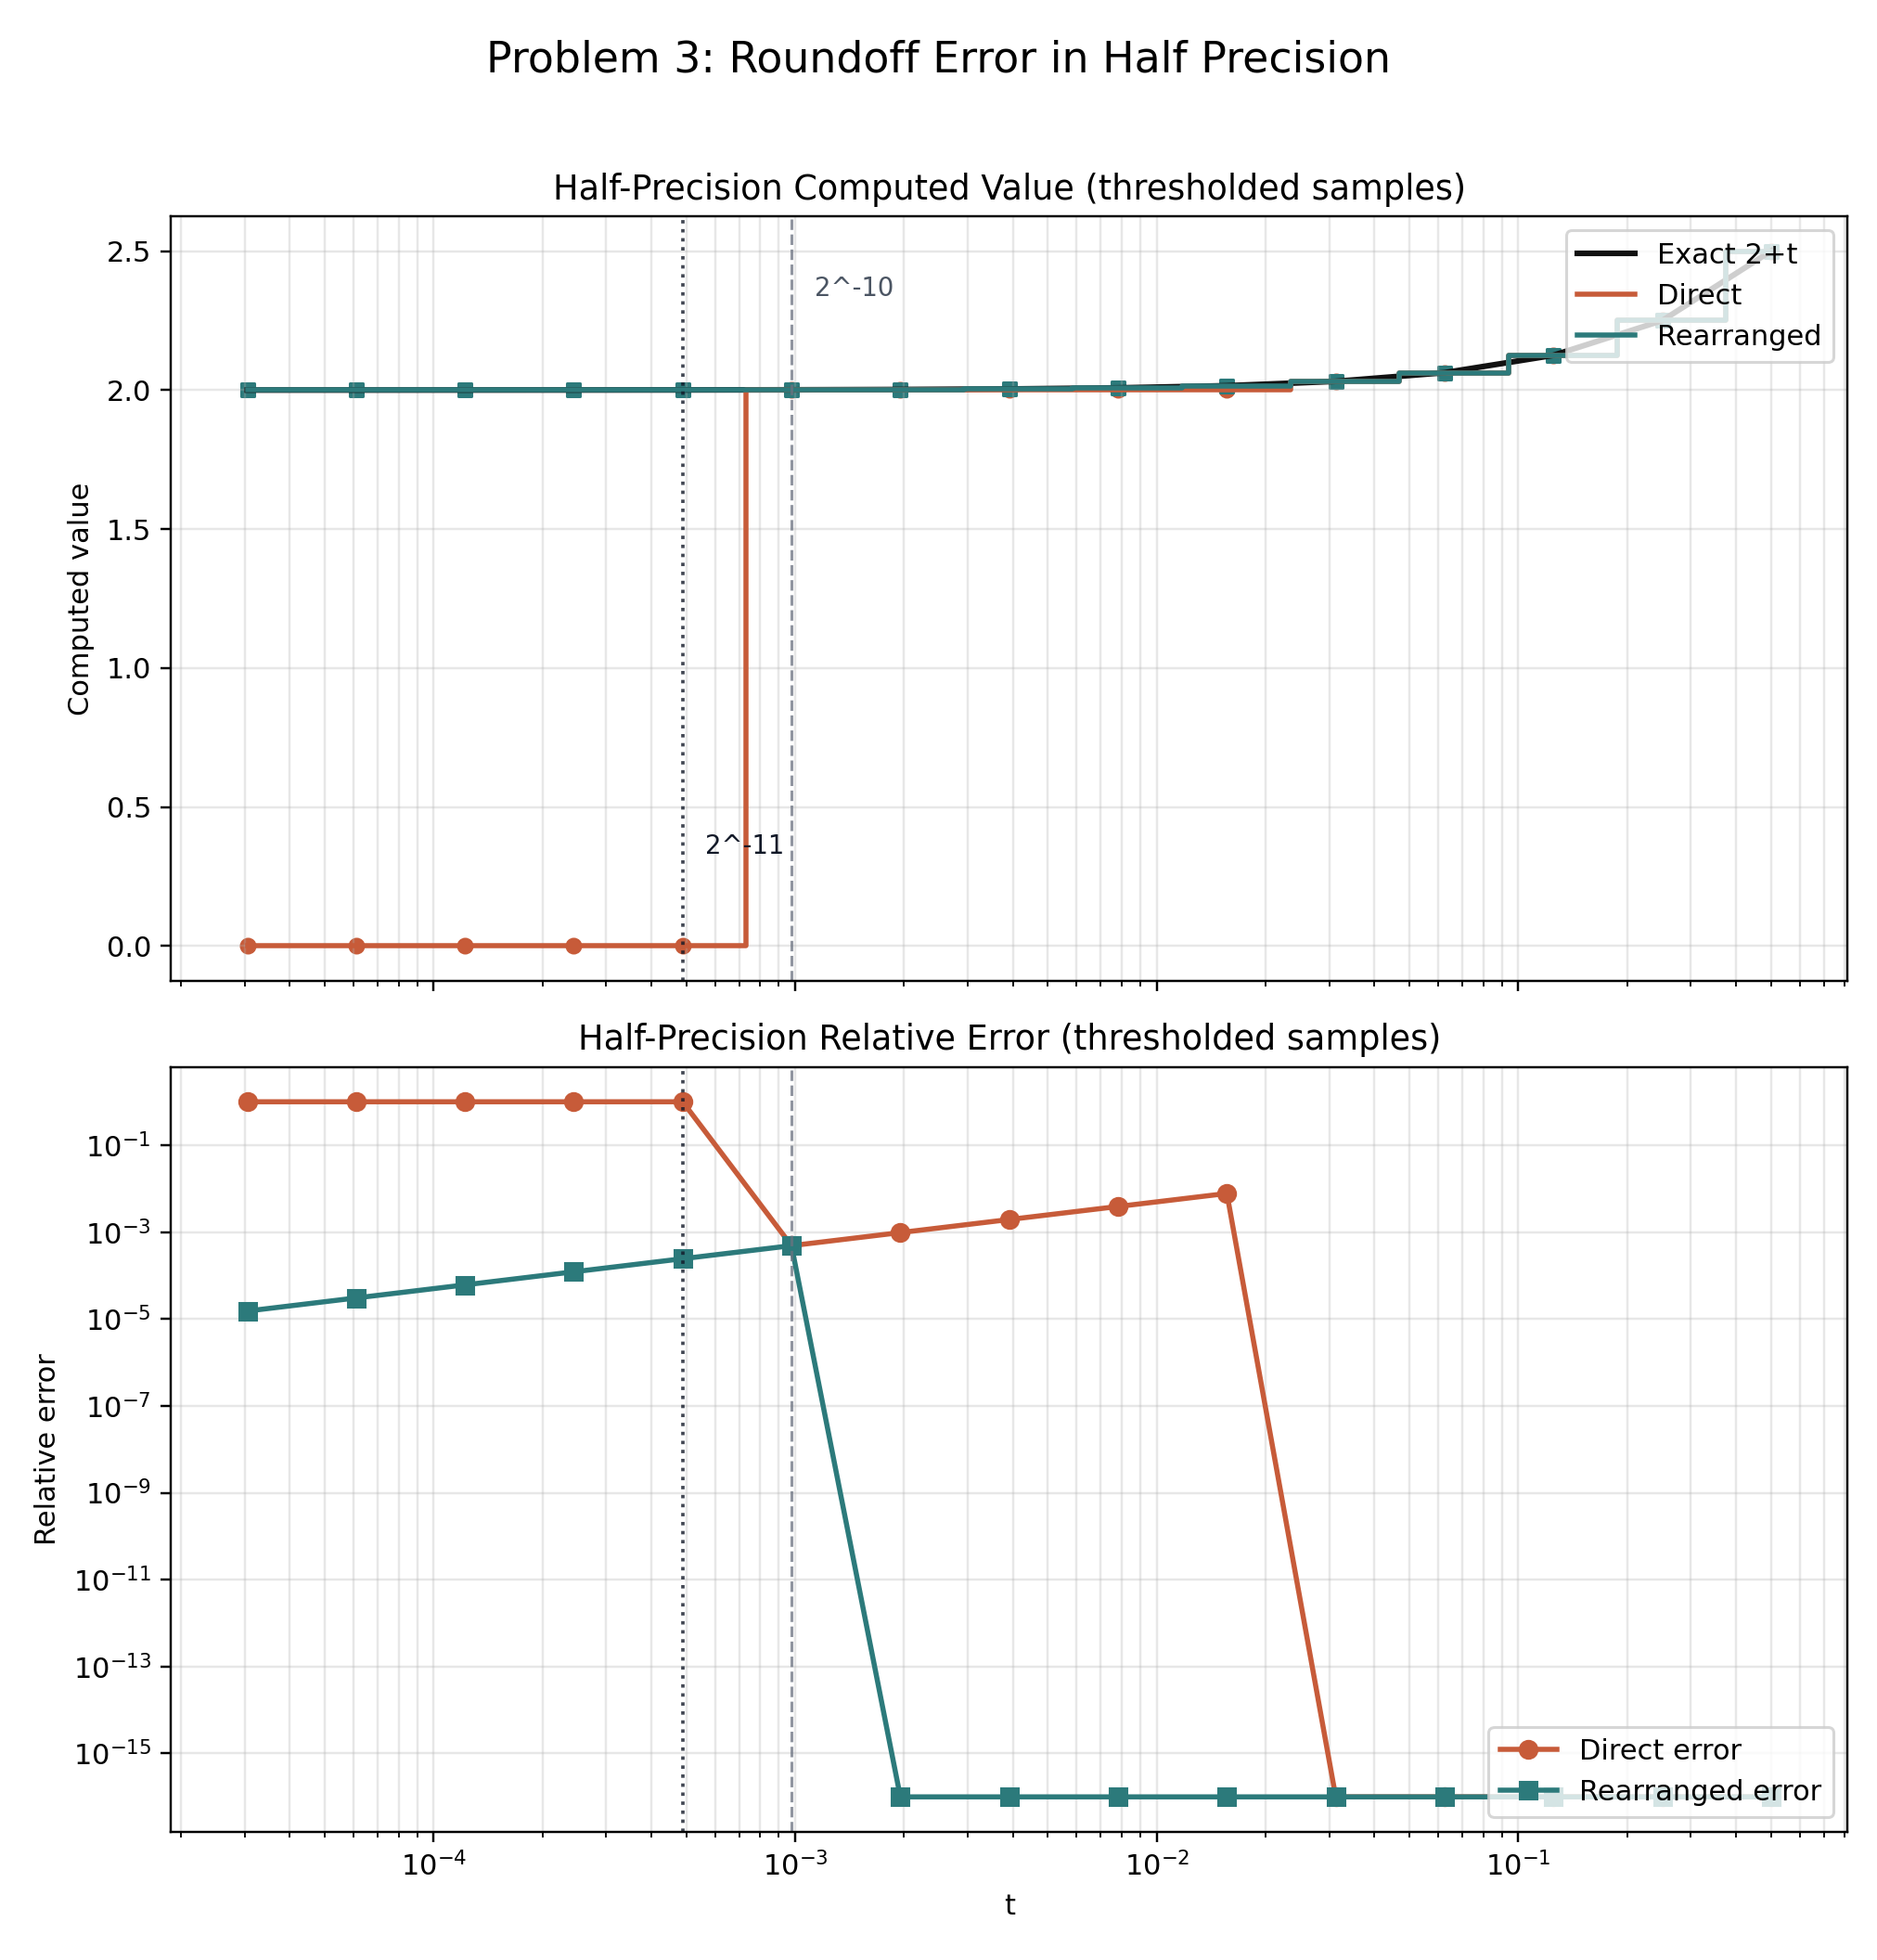
\includegraphics[width=0.88\linewidth,height=0.78\textheight,keepaspectratio,alt={Problem 3 roundoff comparison in half precision}]{../../../result/problem3_roundoff.png}
\caption{Problem 3 roundoff comparison in half precision}
\end{figure}

\blocktitle{分析}

half precision 在 \(1\) 附近的间隔约为 \(2^{-10}\)。当 \(t\) 小于或接近这一阈值时，\(1+t\) 将首先被舍入回 \(1\)，进而使 \((1+t)^2-1\) 被舍入为 \(0\)。本题中的首个失真点正好出现在 \(t=0.00048828125\)，即 machine epsilon 的一半附近，这与 binary16 的舍入行为相一致。由此可见，在低精度格式中，算法结构往往比``理论等价''更重要；对含有相消项的表达式进行代数改写，是避免灾难性误差的关键手段。

\subsection{Problem 3(3)：误差严重程度结论}\label{problem-33ux8befux5deeux4e25ux91cdux7a0bux5ea6ux7ed3ux8bba}

\scriptlink{problem3.c}

\blocktitle{待求问题}

总结 half precision 的 machine epsilon 与舍入误差算例，说明半精度环境下 roundoff error 可达到的严重程度。

\blocktitle{解决方式}

本题采用的实验步骤可归纳为如下伪代码：

\begin{CodeBlock}
Input : half type h, parameter set T
Output: metric table and roundoff plot

probe epsilon(h), min_normal(h)
probe true_min(h), max_finite(h)

for each t in T do
    y_dir <- ((1 + t)^2 - 1) / t
    y_alt <- 2 + t
    y_ref <- high_precision(2 + t)
    if y_ref != 0 then
        err_dir <- relerr(y_dir, y_ref)
        err_alt <- relerr(y_alt, y_ref)
    end if
end for
\end{CodeBlock}

通过比较 \codeinline{y\_dir} 与 \codeinline{y\_alt} 的误差变化，可直接观察 half precision 下的舍入误差放大现象。

\blocktitle{问题答案}

因此，half precision 的 machine epsilon 约为 \(2^{-10}\)，有效数字极为有限；一旦表达式包含相消运算，舍入误差完全可能将本应处于 \(2\) 量级的结果直接压缩为 \(0\)。

\blocktitle{分析}

half precision 在 \(1\) 附近的间隔约为 \(2^{-10}\)。当 \(t\) 小于或接近这一阈值时，\(1+t\) 将首先被舍入回 \(1\)，进而使 \((1+t)^2-1\) 被舍入为 \(0\)。本题中的首个失真点正好出现在 \(t=0.00048828125\)，即 machine epsilon 的一半附近，这与 binary16 的舍入行为相一致。由此可见，在低精度格式中，算法结构往往比``理论等价''更重要；对含有相消项的表达式进行代数改写，是避免灾难性误差的关键手段。

\end{document}
